\documentclass[a4paper,UTF8]{article}
\usepackage{ctex}
\usepackage[margin=1.25in]{geometry}
\usepackage{color}
\usepackage{graphicx}
\usepackage{amssymb}
\usepackage{amsmath}
\usepackage{amsthm}
\usepackage{enumerate}
\usepackage{bm}
\usepackage{hyperref}
\usepackage{pgfplots}
\usepackage{epsfig}
\usepackage{color}
\usepackage{tcolorbox}
\usepackage{mdframed}
\usepackage{lipsum}
\usepackage{framed}
\usepackage{setspace}

\newmdtheoremenv{thm-box}{myThm}
\newmdtheoremenv{prop-box}{Proposition}
\newmdtheoremenv{def-box}{定义}

\setlength{\evensidemargin}{.25in}
\setlength{\textwidth}{6in}
\setlength{\topmargin}{-0.5in}
\setlength{\topmargin}{-0.5in}
% \setlength{\textheight}{9.5in}
%%%%%%%%%%%%%%%%%%此处用于设置页眉页脚%%%%%%%%%%%%%%%%%%
\usepackage{fancyhdr}                                
\usepackage{lastpage}                                           
\usepackage{layout}                                             
\footskip = 10pt 
\pagestyle{fancy}                    % 设置页眉                 
\lhead{2022年秋季}                    
\chead{数字信号处理}                                                
% \rhead{第\thepage/\pageref{LastPage}页} 
\rhead{作业二}                                                                                               
\cfoot{\thepage}                                                
\renewcommand{\headrulewidth}{1pt}  			%页眉线宽,设为0可以去页眉线
\setlength{\skip\footins}{0.5cm}    			%脚注与正文的距离           
\renewcommand{\footrulewidth}{0pt}  			%页脚线宽,设为0可以去页脚线

\makeatletter 									%设置双线页眉                                        
\def\headrule{{\if@fancyplain\let\headrulewidth\plainheadrulewidth\fi%
\hrule\@height 1.0pt \@width\headwidth\vskip1pt	%上面线为1pt粗  
\hrule\@height 0.5pt\@width\headwidth  			%下面0.5pt粗            
\vskip-2\headrulewidth\vskip-1pt}      			%两条线的距离1pt        
 \vspace{6mm}}     								%双线与下面正文之间的垂直间距              
\makeatother  

%%%%%%%%%%%%%%%%%%%%%%%%%%%%%%%%%%%%%%%%%%%%%%
\numberwithin{equation}{section}
%\usepackage[thmmarks, amsmath, thref]{ntheorem}
\newtheorem{myThm}{myThm}
\newtheorem*{myDef}{Definition}
\newtheorem*{mySol}{Solution}
\newtheorem*{myProof}{Proof}
\newtheorem*{myRemark}{备注}
\renewcommand{\tilde}{\widetilde}
\renewcommand{\hat}{\widehat}
\newcommand{\indep}{\rotatebox[origin=c]{90}{$\models$}}
\newcommand*\diff{\mathop{}\!\mathrm{d}}

\usepackage{multirow}

%--

%--
\begin{document}

\title{数字信号处理\\
作业二}
\author{方盛俊\, 201300035} 
\maketitle
%%%%%%%% 注意: 使用XeLatex 编译可能会报错,请使用 pdfLaTex 编译 %%%%%%%

\section*{作业提交注意事项}
\begin{tcolorbox}
\begin{enumerate}
  \item[(1)] 本次作业提交截止时间为~\textcolor{red}{\textbf{2022/12/2  23:59:59}},截止时间后不再接收作业,本次作业记零分;
  \item[(2)] 作业提交方式:使用此~LaTex~模板书写解答,只需提交编译生成的~pdf~文件,将~pdf~文件以ftp方式上传,账号为dsp2022,密码为12345asd!@。请远程连接www.lamda.nju.edu.cn,提交到/D:/courses/DSP2022/HW/HW2路径下。
  \item[(3)] 文件命名方式:学号-姓名-作业号-v版本号, 例~ MG1900000-张三-1-v1;如果需要更改已提交的解答,请在截止时间之前提交新版本的解答,并将版本号加一;
  \item[(4)] 未按照要求提交作业,或~pdf~命名方式不正确,将会被扣除部分作业分数。

\end{enumerate}
\end{tcolorbox}


\newpage
\section{[40pts] 傅里叶级数}
设$x(t)$为某一周期信号。
\begin{enumerate}[(1)]
	\item 设$x(t)=\cos4t+\sin6t+\cos(6t+\displaystyle\frac{\pi}{3}) $,求$x(t)$的\textbf{傅里叶级数}表达式。
	\item 设$x(t)$的部分图像如下所示:\\
	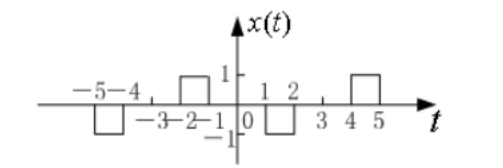
\includegraphics[scale=0.4]{1.png}\\
	求$x(t)$的\textbf{傅里叶级数}表达式。
	\item 设$x(t)$的基波周期为$T_0$,傅里叶级数的系数为$\dot{A}_k$,请用$\dot{A}_k$表示下列傅里叶级数的系数:\\
	(a) $x(t-t_0)$\\
	(b) $x(-t)$\\
	(c) $\displaystyle\int_{-\infty}^tx(\tau)d\tau$,假设$\dot{A}_0=0$\\
	(d) $\displaystyle\frac{dx(t)}{dt}$\\
	(e) $x(at)$,其中$a>0$
\end{enumerate}

\begin{framed}
\begin{spacing}{1.5}
    \begin{itemize}
      \item (1)

      $\displaystyle x(t) = \cos 4t + \sin 6t + \cos(6t+\frac{\pi}{3})$ 的周期为 $\displaystyle \frac{2\pi}{4}$ 和 $\displaystyle \frac{2\pi}{6}$ 的最小公倍数 $\pi$.
      
      $
      \begin{aligned}
      a_0 & = \frac{1}{\pi}\int_{0}^{\pi}[\cos 4t + \sin 6t + \cos(6t+\frac{\pi}{3})]\mathrm{d}t  \\
      & = \frac{1}{\pi}[\frac{1}{4}\sin 4t - \frac{1}{6}\cos 6t + \frac{1}{6}\sin(6t+\frac{\pi}{3})]|_{0}^{\pi}  \\
      & = 0  \\
      \end{aligned}
      $
      
      $
      \begin{aligned}
      a_n & = \frac{2}{\pi}\int_{0}^{\pi}[\cos 4t + \sin 6t + \cos(6t+\frac{\pi}{3})]\cos 2n t \mathrm{d}t  \\
      & = \frac{2}{\pi}\int_{0}^{\pi}[\cos 4t\cos 2n t + (1 - \frac{\sqrt{3}}{2})\sin 6t\cos 2n t + \frac{1}{2}\cos 6t\cos 2n t] \mathrm{d}t  \\
      & = \begin{cases}
          1, & n = 2 \\
          \frac{1}{2}, & n = 3 \\
          0, & \text{otherwise}
      \end{cases}
      \end{aligned}
      $
      
      $
      \begin{aligned}
      b_n & = \frac{2}{\pi}\int_{0}^{\pi}[\cos 4t + \sin 6t + \cos(6t+\frac{\pi}{3})]\sin 2n t \mathrm{d}t  \\
      & = \frac{2}{\pi}\int_{0}^{\pi}[\cos 4t\sin 2n t + (1 - \frac{\sqrt{3}}{2})\sin 6t\sin 2n t + \frac{1}{2}\cos 6t\sin 2n t] \mathrm{d}t  \\
      & = \begin{cases}
          1-\frac{\sqrt{3}}{2}, & n = 3 \\
          0, & \text{otherwise}
      \end{cases}
      \end{aligned}
      $
      
      因此我们也有指数函数族分解系数
      
      $X_n = \begin{cases}X_0 = \frac{1}{2}a_0 \\ X_{-n} = \frac{1}{2}a_n + \frac{j}{2} b_n \\ X_n = \frac{1}{2}a_n - \frac{j}{2} b_n\end{cases} = \begin{cases}
          \frac{1}{4}+j(\frac{1}{2}-\frac{\sqrt{3}}{4}), & n = - 3 \\
          \frac{1}{2}, & n = \pm 2 \\
          \frac{1}{4}-j(\frac{1}{2}-\frac{\sqrt{3}}{4}), & n = 3 \\
      \end{cases}$
      
      因此三角形式傅里叶级数表达式为
      
      $\displaystyle x(t) = \cos 4t + \frac{1}{2}\cos 6t + (1 - \frac{\sqrt{3}}{2})\sin 6t$
      
      因此指数形式傅里叶级数表达式为
      
      $\displaystyle x(t) = [\frac{1}{4}+j(\frac{1}{2}-\frac{\sqrt{3}}{4})]e^{-j 6t} + \frac{1}{2}e^{-j 4t} + \frac{1}{2}e^{j 4t} + [\frac{1}{4}-j(\frac{1}{2}-\frac{\sqrt{3}}{4})]e^{j 6t}$
      
      
      \item (2)
      
      $x(t)$ 的周期为 $T = 6$, 则 $\displaystyle \omega = \frac{2\pi}{T} = \frac{\pi}{3}$.
      
      $\displaystyle a_0 = \frac{1}{6}\int_{-3}^{3}x(t)\mathrm{d}t = \frac{1}{6}\int_{-2}^{-1}-1\mathrm{d}t + \frac{1}{6}\int_{1}^{2}1\mathrm{d}t = - \frac{1}{6} + \frac{1}{6} = 0$
      
      $
      \begin{aligned}
      a_n & = \frac{2}{6}\int_{-3}^{3}x(t)\cos \frac{\pi}{3}nt \mathrm{d}t  \\
      & = \frac{1}{3}\int_{-2}^{-1}\cos \frac{\pi}{3}nt \mathrm{d}t + \frac{1}{3}\int_{1}^{2}-\cos \frac{\pi}{3}nt \mathrm{d}t  \\
      & = \frac{1}{3}\cdot (\frac{3}{\pi n}\sin \frac{\pi}{3}nt)|_{-2}^{-1} + \frac{1}{3}\cdot (-\frac{3}{\pi n}\sin \frac{\pi}{3}nt)|_{1}^{2}  \\
      & = \frac{1}{\pi n}[- \sin{(\frac{\pi n}{3})} + \sin{(\frac{2 \pi n}{3})}] + \frac{1}{\pi n}[\sin{(\frac{\pi n}{3})} - \sin{(\frac{2 \pi n}{3})}]  \\
      & = 0  \\
      \end{aligned}
      $
      
      $
      \begin{aligned}
      b_n & = \frac{2}{6}\int_{-3}^{3}x(t)\sin \frac{\pi}{3}nt \mathrm{d}t  \\
      & = \frac{1}{3}\int_{-2}^{-1}\sin \frac{\pi}{3}nt \mathrm{d}t + \frac{1}{3}\int_{1}^{2}-\sin \frac{\pi}{3}nt \mathrm{d}t  \\
      & = \frac{1}{3}\cdot (-\frac{3}{\pi n}\cos \frac{\pi}{3}nt)|_{-2}^{-1} + \frac{1}{3}\cdot (\frac{3}{\pi n}\cos \frac{\pi}{3}nt)|_{1}^{2}  \\
      & = \frac{1}{\pi n}[- \cos{(\frac{\pi n}{3})} + \cos{(\frac{2 \pi n}{3})}] + \frac{1}{\pi n}[- \cos{(\frac{\pi n}{3})} + \cos{(\frac{2 \pi n}{3})}]  \\
      & = \frac{2}{\pi n}[- \cos{(\frac{\pi n}{3})} + \cos{(\frac{2 \pi n}{3})}]  \\
      \end{aligned}
      $
      
      因此傅里叶级数表达式为
      
      $\displaystyle x(t) = \sum_{n=1}^{\infty}\frac{2}{\pi n}[- \cos{(\frac{\pi n}{3})} + \cos{(\frac{2 \pi n}{3})}]\sin \frac{\pi}{3}n t$
      
      \item (3)
      
      (a)
      
      周期仍然为 $T_0$, 因此 $\omega$ 不变.
      
      $
      \begin{aligned}
      A_k & = \int_{t_1}^{t_1+T_0}x(t-t_0)e^{-jk\omega t}\mathrm{d}t  \\
      & = e^{-jk\omega t_0}\int_{t_1}^{t_1+T_0}x(t-t_0)e^{-jk\omega (t - t_0)}\mathrm{d}(t-t_0)  \\
      & = e^{-jk\omega t_0}\dot{A}_k  \\
      \end{aligned}
      $
      
      (b)
      
      周期仍然为 $T_0$, 因此 $\omega$ 不变.
      
      由于 $\displaystyle x(t) = \sum_{k=-\infty}^{\infty}\dot{A}_k e^{jk\omega t}$
      
      则有 $\displaystyle x(-t) = \sum_{k=-\infty}^{\infty}\dot{A}_k e^{j(-k)\omega t} = \sum_{k'=-\infty}^{\infty}\dot{A}_{-k'} e^{jk'\omega t}$
      
      因此有 $A_k = \dot{A}_{-k}$
      
      (c)
      
      由于 $\displaystyle x(t) = \sum_{k=-\infty}^{\infty}\dot{A}_k e^{jk\omega t}$
      
      则有 $\displaystyle \int_{-\infty}^{t}x(\tau)\mathrm{d}\tau = 0 + \sum_{k=-\infty, k\neq 0}^{\infty}\dot{A}_k (- \frac{j e^{j k \omega t}}{k \omega}) = \sum_{k=-\infty, k\neq 0}^{\infty}- \frac{j \dot{A}_k}{k \omega}e^{j k \omega t}$
      
      因此有 $\displaystyle A_0 = 0, A_k = - \frac{j \dot{A}_k}{k \omega}, k \neq 0$
      
      (d)
      
      由于 $\displaystyle x(t) = \sum_{k=-\infty}^{\infty}\dot{A}_k e^{jk\omega t}$
      
      则有 $\displaystyle \frac{\mathrm{d}x(t)}{\mathrm{d}t} = \sum_{k=-\infty}^{\infty}\dot{A}_k (jk\omega e^{jk\omega t}) = \sum_{k=-\infty}^{\infty}jk\omega \dot{A}_k e^{jk\omega t}$
      
      因此有 $\displaystyle A_k = jk\omega \dot{A}_k$
      
      (e)
      
      周期变为 $\displaystyle T = \frac{T_0}{a}$, 因此 $\omega = a \omega_0$.
      
      由于 $\displaystyle x(t) = \sum_{k=-\infty}^{\infty}\dot{A}_k e^{jk\omega_0 t}$
      
      则有 $\displaystyle x(at) = \sum_{k=-\infty}^{\infty}\dot{A}_k e^{j\omega_0 at} = \sum_{k=-\infty}^{\infty}\dot{A}_k e^{j\omega t}$
      
      因此有 $\displaystyle A_k = \dot{A}_k$
    \end{itemize}
\end{spacing}
\end{framed}


\newpage
\section{[20pts] 傅里叶变换}
求下列信号的傅里叶变换:
\begin{enumerate}[(1)]
	\item $x(t)=e^{-3t}\left[u(t+2)-u(t-3)\right]$
	\item $x(t)=h(t)+h^{\prime}(t)$,其中$h(t)$的图像如下图所示。\\
	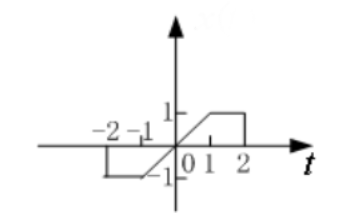
\includegraphics[scale=0.4]{2.png}
\end{enumerate}
	
\begin{framed}
\begin{spacing}{1.5}
    \begin{itemize}
      \item (1)

      由于 $x(t) = e^{-3t}[u(t+2)-u(t-3)]$
      
      $
      \begin{aligned}
      X(j\omega) &= \int_{-\infty}^{+\infty}x(t)e^{-j\omega t}\mathrm{d}t  \\
      &= \int_{-2}^{3}e^{-3t}e^{-j\omega t}\mathrm{d}t  \\
      &= (\frac{1}{-(3+j\omega)}e^{-(3+j\omega) t})|_{-2}^{3}  \\
      &= (\frac{1}{-(3+j\omega)}e^{-3\cdot (3+j\omega)} - \frac{1}{-(3+j\omega)}e^{2\cdot (3+j\omega)})  \\
      &= \frac{1}{3+j\omega}e^{6+j 2\omega} - \frac{1}{3+j\omega}e^{-9-j 3\omega}  \\
      \end{aligned}
      $
      
      \item (2)
      
      由于 $h(t) = \begin{cases}
          -1, & -2 \le t < -1  \\
          t, & -1 \le t < 1  \\
          1, & 1 \le t < 2  \\
          0, & \text{otherwise}
      \end{cases}$
      
      因此有 $x(t) = h(t) + h'(t) = \begin{cases}
          -\delta(t), & t = -2  \\
          -1, & -2 \le t < -1  \\
          t + 1, & -1 \le t < 1  \\
          1, & 1 \le t < 2  \\
          -\delta(t), & t = 2  \\
          0, & \text{otherwise}
      \end{cases}$
      
      $
      \begin{aligned}
      X(j\omega) &= \int_{-\infty}^{+\infty}x(t)e^{-j\omega t}\mathrm{d}t  \\
      &= -e^{j 2\omega} + \int_{-2}^{-1}-e^{-j\omega t}\mathrm{d}t + \int_{-1}^{1}(t+1)e^{-j\omega t}\mathrm{d}t + \int_{1}^{2}e^{-j\omega t}\mathrm{d}t - e^{-j 2\omega}  \\
      &= -e^{j 2\omega} + \frac{1}{j\omega}e^{-j\omega t}|_{-2}^{-1} + (\frac{(j \omega t + j \omega + 1) e^{- j \omega t}}{\omega^{2}})|_{-1}^{1} + \frac{1}{-j\omega}e^{-j\omega t}|_{1}^{2} - e^{-j 2\omega}  \\
      &= -e^{j 2\omega} + \frac{j (e^{j \omega} - 1) e^{j \omega}}{\omega} + \frac{(2 j \omega - e^{2 j \omega} + 1) e^{- j \omega}}{\omega^{2}} + \frac{j (1 - e^{j \omega}) e^{- 2 j \omega}}{\omega} - e^{-j 2\omega}  \\
      &= \frac{1}{\omega^{2}}(- \omega^{2} e^{4 j \omega} - \omega^{2} + j \omega e^{4 j \omega} - j \omega e^{3 j \omega} + j \omega e^{j \omega} + j \omega - e^{3 j \omega} + e^{j \omega}) e^{- 2 j \omega}  \\
      \end{aligned}
      $
    \end{itemize}
\end{spacing}
\end{framed}


\newpage
\section{[20pts] 傅里叶变换的性质 }
设$X(j\Omega)$是下图所示信号$x(t)$的频谱,试在不计算$X(j\Omega)$具体表达式的情况下完成以下计算:
\begin{enumerate}[(1)]
	\item $X(0)$
	\item $\displaystyle\int^{\infty}_{-\infty}X(j\Omega)d\Omega$
	\item $\displaystyle\int^{\infty}_{-\infty}X(j\Omega)\frac{2sin\Omega}{\Omega}e^{j3\Omega}d\Omega$
	\item $\displaystyle\int^{\infty}_{-\infty}\left|X(j\Omega)\right|^2d\Omega$
\end{enumerate}
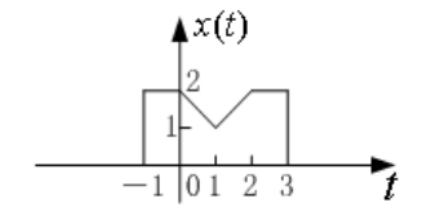
\includegraphics[scale=0.4]{3.png}

\begin{framed}
\begin{spacing}{1.5}
    \begin{itemize}
      \item (1)

      $\displaystyle X(0) = \int_{-\infty}^{+\infty}x(t)\mathrm{d}t = 2 + 1.5 + 1.5 + 2 = 7$
      
      \item (2)
      
      $\displaystyle \int_{-\infty}^{+\infty}X(j\Omega)\mathrm{d}\Omega = 2\pi x(0) = 4\pi$
      
      \item (3)
      
      观察可知 $\displaystyle \frac{2\sin \Omega}{\Omega}$ 为一个矩形信号 $r(t) = \begin{cases}
          A, & |t| \le \frac{\tau}{2} \\
          0, & |t| > \frac{\tau}{2} \\
      \end{cases}$ 的傅里叶变换 $\displaystyle A\tau \cdot \frac{\sin \frac{\Omega \tau}{2}}{\frac{\Omega \tau}{2}}$
      
      因此令 $\displaystyle \frac{\Omega\tau}{2} = \Omega$, $A\tau = 2$ 可得 $\tau = 2$, $A = 1$
      
      令新函数 $\displaystyle y(t) = x(t) * r(t) = \int_{-\infty}^{+\infty}x(\tau)r(t-\tau)\mathrm{d}\tau$
      
      $
      \begin{aligned}
      \displaystyle 2\pi y(3) & = \int_{-\infty}^{+\infty}X(j\Omega)\frac{2\sin \Omega}{\Omega}e^{j 3\Omega}\mathrm{d}\Omega  \\
      & = 2\pi \int_{-\infty}^{+\infty}x(\tau)r(3-\tau)\mathrm{d}\tau  \\
      & = 2\pi \int_{3-1}^{3+1}x(\tau)\mathrm{d}\tau  \\
      & = 2\pi \int_{3-1}^{3}2\mathrm{d}\tau  \\
      & = 4 \pi  \\
      \end{aligned}
      $
      
      \item (4)
      
      $\displaystyle \int_{-\infty}^{+\infty}|X(j\Omega)|^{2}\mathrm{d}\Omega = 2\pi \int_{-\infty}^{+\infty}|x(t)|^{2}\mathrm{d}t = 2\pi(2 \times 4 + 2\int_{1}^{2}t^{2} \mathrm{d}t ) = \frac{76 \pi}{3}$
    \end{itemize}
\end{spacing}
\end{framed}


\newpage
\section{[20pts] 帕斯瓦尔定理 }
\begin{enumerate}[(1)]
    \item 计算
    \begin{equation*}
        \begin{aligned}
        \int^{\infty}_{-\infty}\left(\frac{\sin 2t}{t}\right)^2dt
        \end{aligned}
    \end{equation*}
	\item 证明帕斯瓦尔定理的一般形式:
	\begin{equation*}
        \begin{aligned}
        \int^{\infty}_{-\infty}x(t)y^{*}(t)dt=\frac{1}{2\pi}\int^{\infty}_{-\infty}X(j\Omega)y^{*}(j\Omega)d\Omega
        \end{aligned}
    \end{equation*}
\end{enumerate}

\begin{framed}
\begin{spacing}{1.5}
    \begin{itemize}
      \item (1)

      观察可知 $\displaystyle \frac{\sin 2t}{t}$ 为一个矩形信号 $X(j \Omega) = \begin{cases}
          2\pi A, & |\Omega| \le \frac{\tau}{2} \\
          0, & |\Omega| > \frac{\tau}{2} \\
      \end{cases}$ 的反傅里叶变换 $\displaystyle A\tau \cdot \frac{\sin \frac{t \tau}{2}}{\frac{t \tau}{2}}$
      
      因此令 $\displaystyle \frac{t \tau}{2} = 2t$, $\displaystyle A\tau = 2$ 可得 $\displaystyle \tau = 4$, $\displaystyle A = \frac{1}{2}$, $\displaystyle 2\pi A = \pi$
      
      因此由帕斯瓦尔定理有
      
      $\displaystyle \int_{-\infty}^{+\infty}\left( \frac{\sin 2t}{t} \right)^{2}\mathrm{d}t = \frac{1}{2\pi}\int_{-2}^{2}\pi^{2}\mathrm{d}\Omega = 2 \pi$
      
      \item (2)
      
      $
      \begin{aligned}
      &\quad\ \int_{-\infty}^{\infty}x(t)y^{*}(t)\mathrm{d}t  \\
      &= \int_{-\infty}^{\infty}x(t)[\frac{1}{2\pi}\int_{-\infty}^{\infty}Y^{*}(j\Omega)e^{-j\Omega t}\mathrm{d}\Omega]\mathrm{d}t  \\
      &= \frac{1}{2\pi}\int_{-\infty}^{\infty}Y^{*}(j\Omega)[\int_{-\infty}^{\infty}x(t)e^{-j\Omega t}\mathrm{d}t]\mathrm{d}\Omega  \\
      &= \frac{1}{2\pi}\int_{-\infty}^{\infty}X(j\Omega)Y^{*}(j\Omega)\mathrm{d}\Omega  \\
      \end{aligned}
      $
    \end{itemize}
\end{spacing}
\end{framed}


\newpage
\end{document}